\subsection{RQ3/RQ4: Efficiency, Optimality, Evolution and Stability}
\label{sec:ev-eff}

The last question is operational: what does discovery cost as registries grow, how close is the composition to
the optimum of Eq.~(6), does the QoS objective make the intended trade-offs, and does the engine adapt to
registry changes, failed certificates and repeated requests without losing its guarantees?

\emph{Protocol.} Latency is measured on two virtual CPUs over 30 tasks per registry (measured). Registries of
$10^3$ to $10^5$ tools are built either by cloning the real contracts or by a generator that varies the number of
servers, the mix of effects, the share of private outputs (forbidden pairs), annotation sparsity, the type
vocabulary and duplication. The pairwise risk relation is built in three modes: eager (all pairs, as in the
protocol run), partitioned by effect class, and lazy (decided and cached on demand). Optimality is measured on 80
generated cover instances in eight families against an integer program solved with HiGHS, written independently
of the engine. QoS is tested on 120 instances in which four roles each have four interchangeable providers with
different price, latency and failure rate, so that all 256 toolkits and their exact Pareto front can be
enumerated. Evolution replays the removal and re-insertion of each of the 76 servers; refinement uses the test
tasks; experience reuse replays 300 requests against a pattern repository with mandatory revalidation.

\begin{table}[t]
\centering
\caption{Engine build time by pair-relation mode (cloned registries; eager at $10^5$ from the protocol run) and
request latency over 30 tasks (two virtual CPUs); last column: heterogeneous registries, lazy mode.}
\label{tab:ev-scale}
\scriptsize
\setlength{\tabcolsep}{3pt}
\begin{tabular}{@{}rrrrrrrr@{}}
\toprule
 & \multicolumn{3}{c}{Build (s)} & \multicolumn{2}{c}{Latency (ms)} & & Het. \\
\cmidrule(lr){2-4}\cmidrule(lr){5-6}
Tools & eager & part. & lazy & p50 & p95 & Abst. & p50 \\
\midrule
569 & 2.2 & 2.6 & 2.5 & 49 & 191 & 2/30 & -- \\
1,000 & 2.8 & 3.0 & 3.0 & 58 & 786 & 3/30 & 44 \\
10,000 & 30.3 & 14.5 & 14.4 & 281 & 5689 & 9/30 & 192 \\
100,000 & 2223.7 & 134.5 & 133.4 & 2669 & 16098 & 10/30 & 3207 \\
\bottomrule
\end{tabular}
\end{table}


\begin{figure*}[t]
\centering
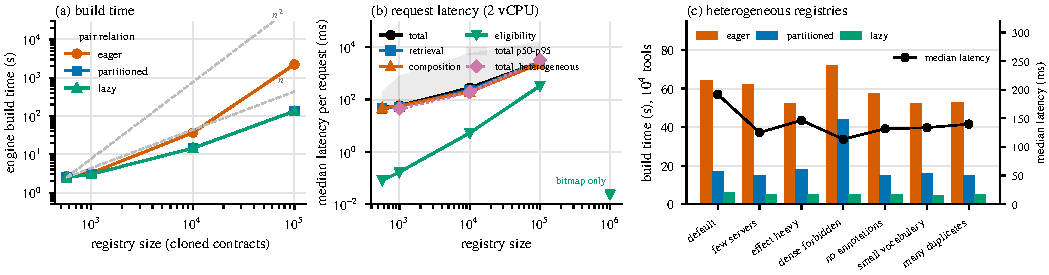
\includegraphics[width=\textwidth]{fig_eff_scale}
\caption{Scalability. (a) Engine build time against registry size for the three pair-relation modes (cloned
contracts; dashed: linear and quadratic references). (b) Median request latency by stage (band: total p50--p95),
heterogeneous registries, and the bitmap eligibility test alone at $10^6$ contracts. (c) Build time and latency at
$10^4$ tools for each heterogeneous factor.}
\label{fig:ev-scale}
\end{figure*}

\emph{Scalability.} On the real registry a request takes 49\,ms at the median (191\,ms at the 95th percentile):
eligibility 0.08\,ms, per-goal retrieval 45\,ms, against 12\,ms for one dense ranking of the request (RAG-MCP).
The median grows to 58\,ms at $10^3$ cloned tools, 281\,ms at $10^4$ and 2.7\,s at $10^5$ (16.1\,s at the 95th
percentile), almost all of it retrieval and composition (Fig.~\ref{fig:ev-scale}b); the bitmap test alone takes
0.024\,ms over $10^6$ contracts, an index measurement that does not extend to the full engine. Building the engine
was the bottleneck of the protocol run, which materialises the pairwise risk relation eagerly: 2,224\,s at $10^5$
tools (Table~\ref{tab:ev-scale}). Partitioning the relation by effect class or deciding it lazily gives
identical toolkits on all 94 test tasks and builds in 134 and 133\,s at $10^5$ tools, 16.5 times faster, with a
growth close to linear (Fig.~\ref{fig:ev-scale}a). On heterogeneous registries of $10^4$ tools the lazy mode
builds in 4.6--5.9\,s whatever the factor, while the partitioned mode depends on the density of forbidden pairs
(43.9\,s when half of the outputs are private) and the eager mode takes 52--72\,s (Fig.~\ref{fig:ev-scale}c);
median latency stays between 113 and 192\,ms. At $10^5$ heterogeneous tools the lazy engine builds in 57\,s and
answers in 3.2\,s at the median. Two concurrent workers serve 21.0 requests per second against 11.3 for one.

\begin{table}[t]
\centering
\caption{Composition against exact optima (integer program, HiGHS) on 80 generated cover instances, ten per
family: infeasible instances, abstentions agreeing with the ILP, exact search equal to the optimum among the
instances it solved, node-budget exhaustion, greedy excess cost (mean, max; \%) and median times (ms).}
\label{tab:ev-opt}
\scriptsize
\setlength{\tabcolsep}{2.2pt}
\begin{tabular}{@{}lrrrrlrrr@{}}
\toprule
Family & Inf. & Abst. & Exact & Budget & Greedy (\%) & Exact & Greedy & ILP \\
\midrule
base & 0 & 10/10 & 10/10 & 0 & 4.4 (17.2) & 31 & 7 & 0.9 \\
6 alternatives & 0 & 10/10 & 10/10 & 0 & 5.4 (17.1) & 998 & 10 & 9.4 \\
depth 3 & 0 & 10/10 & 10/10 & 0 & 8.0 (36.6) & 186 & 11 & 7.3 \\
arity 2 & 0 & 10/10 & 10/10 & 0 & 7.2 (20.6) & 33 & 7 & 6.6 \\
conflicts & 0 & 10/10 & 10/10 & 0 & 12.0 (43.2) & 77 & 8 & 8.6 \\
shared tools & 0 & 10/10 & 10/10 & 0 & 12.6 (26.8) & 370 & 10 & 6.8 \\
6 goals & 0 & 10/10 & 1/1 & 9 & 6.9 (21.1) & 6703 & 22 & 6.1 \\
infeasible & 10 & 10/10 & 0/0 & 0 & -- & 3 & 3 & 1.1 \\
\bottomrule
\end{tabular}
\end{table}


\begin{figure*}[t]
\centering
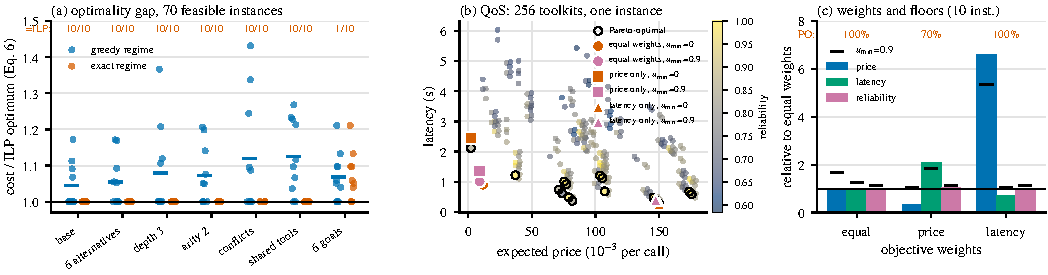
\includegraphics[width=\textwidth]{fig_eff_opt}
\caption{Optimality and QoS. (a) Cost of the greedy and exact regimes relative to the ILP optimum per instance
family (top: instances where the exact search equals the optimum; with six goals the exact regime exhausts its
budget and falls back to greedy in nine instances). (b) All 256 toolkits of one QoS instance with their Pareto front
and the toolkits chosen under three weightings and two utility floors. (c) Mean price, latency and reliability of
the chosen toolkits relative to equal weights (bars: $u_{\min}=0$, ticks: $u_{\min}=0.9$; PO: share
Pareto-optimal).}
\label{fig:ev-opt}
\end{figure*}

\emph{Optimality.} Wherever the exact search finishes, it returns the ILP optimum: in all 61 solved instances,
across alternative counts, depths, arities, conflict densities and shared tools (Table~\ref{tab:ev-opt}), and the
optimum over the candidate set equals the optimum over all tools, so candidate truncation lost nothing on these
instances. All ten infeasible instances are recognised, and abstentions agree with the ILP in all 80. The greedy
regime is 4.4--12.6\% above the optimum on average and up to 43.2\% (conflicts; Fig.~\ref{fig:ev-opt}a). With six
goals the exact search exhausts its 20,000-node budget in nine of ten instances after 6.7\,s and falls back to the
greedy regime, 6.9\% above the optimum on average, without any guarantee; the ILP solves every family's instances in 1--9\,ms at
the median, which makes it the better exact back-end for larger covers.

\emph{QoS trade-offs.} The QoS objective acts as intended once providers differ (Fig.~\ref{fig:ev-opt}b,c). With
equal weights every chosen toolkit is Pareto-optimal and meets the utility floor; weighting price alone lowers the
mean price to 0.33 times at 2.1 times the latency, weighting latency alone lowers latency to 0.73 times at 6.6 times
the price, and a floor of 0.9 raises mean reliability from 0.84 to 0.93 at 1.7 times the price. Two limits appear.
With price alone only 70\% of the choices are Pareto-optimal, because ties in price are broken without regard to
latency; and because Eq.~(6) normalises price and latency before weighting them, the equal-weight choice is 32\%
above the optimum of the same weighted sum in raw units. On the benchmark registries, which publish no QoS data,
price and latency weights change no toolkit; the evidence and token weights change 7.2--20.1\% and 2.9--7.2\% of
them, with recall between 0.197 and 0.215.

\begin{figure*}[t]
\centering
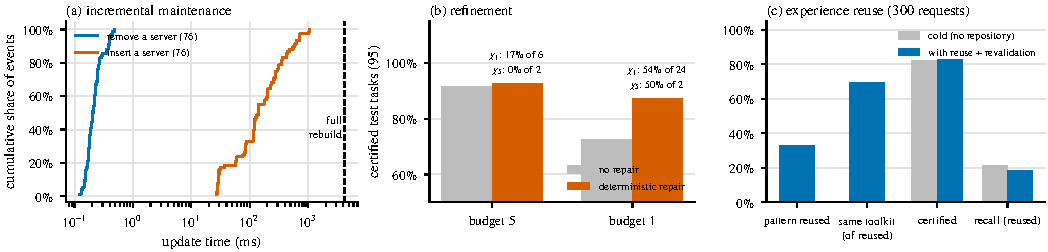
\includegraphics[width=\textwidth]{fig_eff_evolution}
\caption{Adaptation. (a) Distribution of incremental update times when each of the 76 servers is removed and
re-inserted, against a full rebuild. (b) Certified test tasks before and after the deterministic repair
operators, at the default candidate budget and with $\chi_1$ counterexamples induced by a budget of one (labels:
share of each counterexample class repaired). (c) Experience reuse with revalidation against cold discovery.}
\label{fig:ev-evolution}
\end{figure*}

\emph{Evolution.} Replaying 152 server removals and insertions, an incremental update takes 13.5\,ms at the
median (565\,ms at the 95th percentile, insertions dominating) against 4.2\,s for a rebuild
(Fig.~\ref{fig:ev-evolution}a). The exact invalidation rule of Proposition~3 invalidates 1.1\% of the 35 cached
toolkits per event instead of all of them, and after the replay 33 of the 35 recomputed toolkits equal the
originals. All 20 simulated rug pulls lose their observed evidence and regain it when the verified definition
returns; with the drift measured on the reference servers (Section~\ref{sec:ev-rq2}) this mechanism would fire on
every one of their tools.

\emph{Refinement.} On the 95 test tasks, 91.6\% are certified at once; the deterministic repair operators raise
this to 92.6\%, repairing one of six $\chi_1$ and neither $\chi_5$ counterexample. With $\chi_1$ induced by a
candidate budget of one, they raise certification from 72.6\% to 87.4\%, repairing 54\% of the 24 $\chi_1$ and one
of two $\chi_5$ (Fig.~\ref{fig:ev-evolution}b); the revenue scenario of Fig.~3 is repaired by the $\chi_5$ split.
LLM-proposed repairs were not evaluated.

\emph{Experience reuse.} Over 300 requests the repository stores 158 patterns and reuses one for 98 requests
(32.7\%), each saving an analyst call (Fig.~\ref{fig:ev-evolution}c). After the mandatory revalidation, 69.4\% of
the reused toolkits equal the cold ones, certification is unchanged (82.7\% against 82.3\%), recall on the reused
requests is slightly lower (0.184 against 0.214). Revalidation was probed on 89 reused requests by changing the
state after storage: removing the pattern's servers, revoking or rewriting its tools' definitions, applying a
strict read-only principal, or switching to Haiku's profile; no revalidated toolkit violated the changed state
(the stricter principal led to 5 abstentions). Because analyst calls are replayed here, the latency saving of reuse
is not visible (18.3 against 17.7\,ms); its benefit is the avoided LLM call.

\begin{table}[t]
\centering
\caption{Confirmatory comparisons, fixed before the data they test (F1--F7 before the set-level experiments; H1--H5
in a dated amendment before the revised test runs), Holm-corrected within each family. Differences in points
(tokens for F6), \pamcp{} minus comparator, with 95\% CI.}
\label{tab:ev-family}
\scriptsize
\setlength{\tabcolsep}{2.2pt}
\begin{tabular}{@{}llrlll@{}}
\toprule
 & Comparison & $\Delta$ & 95\% CI & $p_{\mathrm{Holm}}$ & Verdict \\
\midrule
F1 & Group recall vs per-subtask (non-inf., 0.05) & -8.0 & [-16.6, +0.2] & 1.000 & not shown \\
F2 & Size-matched recall vs RAG-MCP & +6.0 & [-1.6, +13.7] & 0.397 & n.s. \\
F3 & Joint feasibility vs per-subtask (elig.) & +4.3 & [-8.5, +18.1] & 1.000 & n.s. \\
F4 & Exp@5 verified vs lexical & -9.9 & [-13.9, -6.6] & $<$0.001 & supports \\
F5 & Reachable attacks vs per-subtask & -2.7 & [-3.9, -1.5] & $<$0.001 & supports \\
F6 & Tokens, full vs NoGap & -16.7 & [-34.6, +1.0] & 0.269 & n.s. \\
F7 & Hit@1 goal contract vs raw RRF (569) & -15.7 & [-21.3, -10.0] & $<$0.001 & against \\
\midrule
H1 & Hit@1 PaMCP-L vs tuned BM25 (569) & +0.3 & [-8.9, +8.8] & 1.000 & n.s. \\
H2 & Hit@1 PaMCP-L vs Eq. (5) (569) & +11.7 & [+3.0, +22.6] & 0.070 & n.s. \\
H3 & Group recall PaMCP-L vs per-subtask (non-inf.) & -8.8 & [-17.6, -0.5] & 1.000 & not shown \\
H4 & Strict joint feas. vs per-subtask (elig.) & +7.4 & [+0.0, +14.9] & 0.277 & n.s. \\
H5 & Definite out-of-scope vs per-subtask & -20.0 & [-28.4, -12.6] & $<$0.001 & supports \\
\bottomrule
\end{tabular}
\end{table}


\emph{Statistical stability.} With 300 requests on 66 target tools, intervals that resample target tools are 2.7
to 3.3 times wider than request-level ones, so request-level intervals would overstate precision; all intervals
above resample clusters. The ranking of the retrieval methods is stable across category-stratified half splits
(Kendall's $\tau=0.68$, the same best method in all 200 splits) and less so across tool-disjoint splits
($\tau=0.43$, 87.5\%); these resamples measure stability of one sample, not replication on new data.
Table~\ref{tab:ev-family} collects the confirmatory comparisons. Four favour \pamcp{} after correction: exposure
against lexical cues (F4), reachable attacks (F5) and definite out-of-scope attacks (H5), all security outcomes,
and none on retrieval or recall. One goes against it (F7, single-tool retrieval with Eq.~(5)), non-inferiority of
recall is shown for neither variant (F1, H3), and the remaining five are not significant.

\emph{Interpretation.} The full engine scales to $10^5$ tools at second-level latency once the risk relation is
not materialised eagerly, which the revision shows to be an implementation choice rather than a property of the
model; the exact search is optimal where it finishes but should hand larger covers to an ILP solver; and the QoS
objective makes Pareto-optimal trade-offs when the registry provides QoS data, which the benchmark registries do
not. Evolution is cheap and exact, deterministic repair recovers induced counterexamples but rarely natural ones,
and reuse saves LLM calls without weakening certification.
